\vspace{-4mm}
\begin{figure*}[!ht]
    \centering
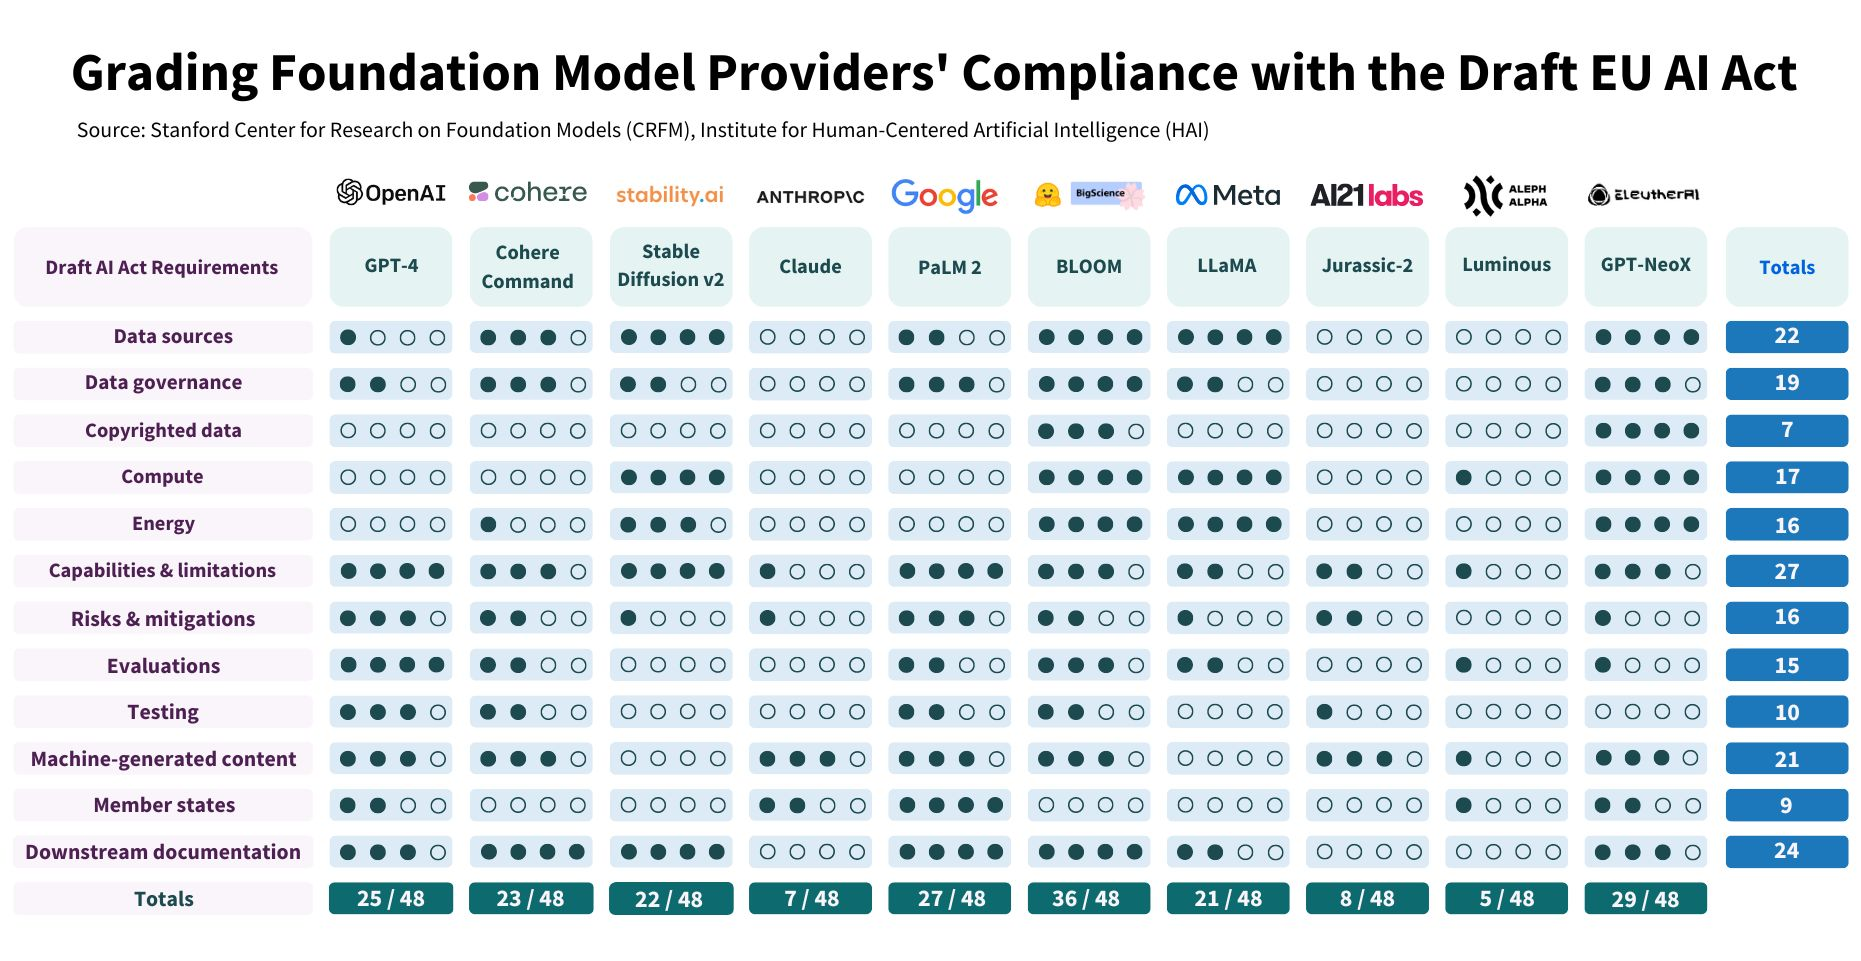
\includegraphics[width=\textwidth]{img/EU_grading.jpeg}
%\vspace{-2mm}
\caption{Grading of current LLMs as proposed by a report entitled \emph{Do Foundation Model Providers Comply with the EU AI Act?} from Stanford University \cite{bommasani2023eu-ai-act}.}
\label{fig:HAI_grading}
\end{figure*}
\vspace{-2mm}

\newpage
\section{Discussion and Limitations}
\vspace{-2mm}
\textbf{Discussion:} On June 14\textsuperscript{th}, 2023, the European Parliament successfully passed its version of the EU AI Act \cite{euaiproposal}. Subsequently, a team of researchers from the Stanford Institute for Human-Centered Artificial Intelligence (HAI) embarked on investigating the extent to which Foundation Model Providers comply with the EU AI Act. Their initial findings are presented in the publication \cite{bommasani2023eu-ai-act}. In this study, the authors put forward a grading system consisting of 12 aspects for evaluating LLMs. These aspects include \emph{(i) data sources, (ii) data governance, (iii) copyrighted data, (iv) compute, (v) energy, (vi) capabilities \& limitations, (vii) risk \& mitigations, (viii) evaluation, (ix) testing, (x) machine-generated content, (xi) member states, and (xii) downstream documentation}. The overall grading of each LLM can be observed in \cref{fig:HAI_grading}. While this study is commendable, it appears to be inherently incomplete due to the ever-evolving nature of LLMs. Since all scores are assigned manually, any future changes will require a reassessment of this rubric, while HVI is auto-computable. Furthermore, we propose that HVI should be considered the most suitable category for assessing risk and mitigations, as well as the evaluation of machine-generated content.

\textbf{Limitations:} In this paper, we present a unique and extensive benchmark corpus for hallucination called 
\includegraphics[height=0.3cm,width=1cm]{img/hilt.png}. We propose two main types of hallucination: (i) Factual Mirage and (ii) Silver Lining, each further divided into intrinsic and extrinsic sub-categories. Additionally, we introduce six detailed categories of hallucination along with a measure of its intensity. We believe the following aspects require critical attention in future endeavors.


\textbf{Limitation 1:} For the sake of simplicity, we have only considered one category per sentence during annotation, although we acknowledge the presence of multi-class and multi-label instances. For instance, in the following example, there are two kinds of hallucination, namely Time Wrap and Numeric Nuisance present in the shown sentence. We would like to explore this direction in the immediate future. 

\vspace{-3mm}

\begin{tcolorbox}[enhanced,attach boxed title to top right={yshift=-2.5mm,yshifttext=-1mm}, left=1pt,right=1pt,top=1pt,bottom=1pt,
  colback=blue!5!white,colframe=blue!75!black,colbacktitle=red!80!black,
  title=alarming,fonttitle=\ttfamily\bfseries\scshape\fontsize{9}{9.6}\selectfont,
  boxed title style={size=fbox,colframe=red!50!black} ]
    \label{tab:misc}
    %\vspace{-2mm}
  \begin{spacing}{0.75}
  \textbf{\scriptsize Prompt:} \textit{\scriptsize Engineering effort to build Eiffel tower}
  \end{spacing}

  \vspace{-2mm}
  \DrawLine

  \begin{spacing}{0.75}
  \textbf{\scriptsize AI-generated text:} {\fontfamily{lmss}\scriptsize\selectfont
  ...Designed by Gustave Eiffel, it was inaugurated in 1889 to celebrate the \textcolor{red}{100th anniversary of the European Civil War}, while construction began \textcolor{blue}{a decade prior to its inauguration}....}
  \end{spacing}

  \vspace{-2mm}
  \DrawLine

  %\begin{spacing}{0.75}
  \textbf{\scriptsize Fact 1:} \scriptsize Eiffel tower was built to celebrate the 100th anniversary of the French Revolution.\\
  \textbf{\scriptsize Fact 2:} \scriptsize Eiffel Tower construction was started in 1887, not in 1879.
  %\end{spacing}

  %\vspace{-1mm}
\end{tcolorbox}
%\vspace{-1mm}

\textbf{Limitation 2:} While we have meticulously defined the categories of hallucination, we recognize the potential for new categories to emerge in the future with the advancement of LLMs. An instance of this is the introduction of name-nationality hallucination by \citep{ladhak2023pre}, where a person named Jung Lee is falsely attributed with French nationality. Although one could argue that Mr Lee may indeed be a French national, considering his birth and upbringing there, the authors confirm that no such individual exists. We posit that name-nationality hallucination falls under the sub-class of generated golems. It is plausible that a combination of our defined categories may exist, although we did not extensively studied these possibilities.
%Although we have defined the categories of hallucination in a fine-grained and holistic manner, we acknowledge the possibility of additional categories emerging with the advent of new LLMs in the future. For example \citep{ladhak2023pre} introduced name-nationality hallucination. For example, a person name Jung Lee has been assigned French nationality. While it could be argued that possibly Mr Lee is a French national and was born and grew up there, unfortunately, no such personality exists, as confirmed by the authors. We argue that name-nationality hallucination is a sub-class of the generated golem. It is quite possible mixture of our defined categories may exist, but we did not do an extensive study on this. 

\textbf{Limitation 3:} For this study, we have chosen 15 contemporary LLMs. In the dynamic landscape of LLM development, new models are constantly emerging, and we acknowledge that our selection may not encompass all available options. Keeping this in mind, we will make the 
\includegraphics[height=0.3cm,width=1cm]{img/hilt.png} benchmark and the \textit{HVI} publicly accessible for collaborative updates and contributions.

\textbf{Limitation 4:} The FACTUALITY\textsubscript{GB} technique operates based on entailment, allowing it to distinguish between sentences containing different entities such as \emph{Barack Obama} and \emph{Joe Biden.} However, it is unable to differentiate sentences that involve similar entities like \emph{AI} and \emph{AAAI.} In contrast, the ENTROPY\textsubscript{BB} technique operates at the token level and is capable of handling cases like \emph{1789} vs. \emph{1889.} These distinctions become evident in the observed results.

%Some AI-generated texts can belong to multiple hallucination categories, such an example has been provided in \cref{tab:multipleH}. However, in this work, we only consider one category for each sentence. 

\section{Ethical Considerations}
Through our experiments, we have uncovered the susceptibility of LLMs to hallucination. In developing HVI, we intend to provide a framework that can inform future research and policies in this domain. However, we must address the potential misuse of our findings by malicious entities who may exploit AI-generated text, such as creating indistinguishable fake news from human-written content. We vehemently discourage such misuse and strongly advise against it.






